\documentclass[conference]{IEEEtran}
\usepackage{cite}
\usepackage{amsmath,amssymb}
\usepackage{graphicx}
\usepackage{booktabs}
\usepackage{algorithm}
\usepackage{algpseudocode}
\usepackage{url}
\usepackage{hyperref}
\usepackage{xcolor}
\graphicspath{{figures/}}

\begin{document}

\title{TrialMatch-KV: Evidence-Grounded Clinical-Trial Criterion Matching with a LoRA-Fine-Tuned Qwen2.5 Transformer and Hand-Written KV-Cache, Tiled-Attention and Speculative-Decoding Inference}

\author{\IEEEauthorblockN{Muhammad Ali}
\IEEEauthorblockA{\textit{Roll No.\ 23i-0008, Section B} \\
\textit{Generative AI -- Assignment \#2} \\
\textit{[Department, University]}, [City, Country] \\
m.alenauman@gmail.com \\
Source code: \url{https://github.com/Ali-prog-spec/TrialMatch-KV}}}

\maketitle

\begin{abstract}
We build and evaluate a complete, locally executable system that judges whether a patient description satisfies an individual inclusion or exclusion criterion of a clinical trial and cites the supporting patient sentences. A Qwen2.5-1.5B-Instruct decoder is adapted with LoRA on the patient-grouped training split (37/8/8 patients, seed 42) of the TrialGPT Criterion Annotations. On the untouched test split (206 criteria, 8 patients) a first LoRA adapter (v1) raises accuracy from 0.223 to 0.723 but collapses to the majority label (``not excluded'') on all 131 exclusion criteria (macro-F1 0.379). A second adapter (v2), trained with class-balanced sampling and selected by validation macro-F1 only, reaches accuracy 0.718, macro-F1 0.486 and evidence micro-F1 0.543 (base: 0.223, 0.211, 0.144), and begins to predict the rare classes. On the inference side we implement from scratch (i) a KV-cached greedy decoder with explicit positions and cache updates, verified token-identical to an uncached reference in nine length configurations with 2.0--8.1$\times$ speed-ups (one 38.7$\times$ outlier we could not explain), (ii) reference and tiled online-softmax attention that agree within $10^{-6}$ (fp32), and (iii) greedy speculative decoding that is token-identical to greedy decoding in all 12 tests but, on our hardware, 0.49--1.00$\times$ the speed of plain greedy decoding. Everything is exposed through a browser application with per-criterion evidence, an exportable report and a live decoder comparison. The system is an educational screening prototype, not a clinical decision tool.
\end{abstract}

\begin{IEEEkeywords}
clinical trial matching, eligibility criteria, LoRA, KV cache, online softmax, speculative decoding, evidence retrieval
\end{IEEEkeywords}

\section{Introduction}
Matching patients to clinical trials requires reading free-text eligibility criteria and deciding, for each criterion, whether the patient meets it. Large proprietary models such as GPT-4 have been shown to do this reasonably well \cite{jin2024trialgpt}, but they are costly and cannot be run privately on patient text. This work asks a narrower, reproducible question: \emph{how far can a small open-weight decoder (1.5B parameters, 6\,GB consumer GPU) be adapted to the criterion-level task, and can we implement and measure the inference mechanisms that make such a model practical?}

The assignment decomposes into six tasks, each answered in this paper: (1) research-driven model selection and fine-tuning; (2) criterion-level eligibility classification with evidence verification that keeps the dataset's label categories (including \emph{not enough information} and \emph{not applicable}); (3) a KV-cached decoding path with an uncached reference; (4) tiled online-softmax attention; (5) greedy speculative decoding; and (6) an integrated browser application. We deliberately report negative results (majority-class collapse on exclusion criteria, speculative-decoding slowdown, a slow tiled kernel) rather than hiding them.

\section{Related Work}
\textit{Clinical-trial matching.} TrialGPT \cite{jin2024trialgpt} uses GPT-4 to produce criterion-level eligibility labels, supporting sentences and explanations, and aggregates them into trial scores; its released criterion annotations by clinicians are the benchmark used here. We study the repository only as a reference; all training, evaluation and inference code is our own, and the GPT-4 predictions contained in the dataset are never used as inputs.

\textit{Parameter-efficient adaptation.} LoRA \cite{hu2022lora} freezes the base weights and learns low-rank updates $\Delta W = BA$, which fits our memory budget (a 1.5B model in fp16 needs 3.1\,GB; full fine-tuning with Adam states would not fit in 6\,GB).

\textit{Decoder architectures.} We use the Qwen2.5 family \cite{qwen25}: pre-norm decoder-only Transformers with rotary position embeddings (RoPE) \cite{su2021roformer}, grouped-query attention, SwiGLU feed-forward layers and RMSNorm \cite{vaswani2017attention} for the base design.

\textit{Efficient attention.} Online (streaming) softmax \cite{milakov2018online} computes softmax with a running maximum and normaliser; FlashAttention \cite{dao2022flashattention} combines it with tiling so the $T\times T$ score matrix is never materialised. KV caching and its memory management in serving systems are discussed in \cite{kwon2023pagedattention}.

\textit{Speculative decoding.} A small draft model proposes tokens that the large model verifies in one parallel pass \cite{leviathan2023speculative,chen2023accelerating}; under greedy decoding the output equals that of the target alone.

\section{Materials and Methods}
\subsection{Dataset and fixed split}
We use only \texttt{ncbi/TrialGPT-Criterion-Annotations}: 1015 criterion-level annotations over 53 patients. Inputs are the patient note (numbered sentences), the criterion type and the criterion text. The expert label (inclusion: \emph{included, not included, not enough information, not applicable}; exclusion: \emph{excluded, not excluded, not enough information, not applicable}) and expert evidence sentence IDs are the targets. Columns \texttt{gpt4\_*}, \texttt{explanation\_correctness} and the original \texttt{training} flag are never read. One record (annotation 883) has a null criterion text in the source dataset; we keep it and substitute an explicit placeholder so that split counts are unchanged.

The split follows the prescribed protocol: unique patient IDs are sorted, shuffled with \texttt{numpy.random.default\_rng(42).shuffle}, and the first 37, next 8 and last 8 patients form train, validation and test (603, 206 and 206 annotations). A manifest (\texttt{data/split\_manifest.json}) lists all patient IDs, and an assertion checks that no patient appears in two splits. The test split was evaluated once, after all choices were frozen on validation data.

Label distribution is strongly skewed: of 659 exclusion annotations in the whole set, 484 are \emph{not excluded} and only 10 are \emph{excluded}; 610 of 1015 annotations (60\%) have no expert evidence sentence. Both facts shape the results (Sec.~\ref{sec:results}).

\subsection{Research-driven model selection}
Candidates (parameter counts and licences from the official model cards) were: \textbf{Qwen2.5-1.5B-Instruct} (1.54B params incl.\ embeddings, 28 layers, hidden 1536, 12 query / 2 KV heads, vocabulary 151\,936, 32\,k context, Apache-2.0) \cite{qwen25}; Llama-3.2-1B-Instruct (1.24B, 128\,k context, Llama community licence, gated download); SmolLM2-1.7B-Instruct (1.7B, 8\,k context, Apache-2.0); and Phi-3-mini (3.8B, MIT, too large to LoRA-train in fp16 on 6\,GB). We selected Qwen2.5-1.5B because (a) 3.1\,GB of fp16 weights plus LoRA training state fits in 6\,GB (measured peak 4.34\,GB with gradient checkpointing), (b) its permissive licence and non-gated weights make the repository reproducible, (c) the 32\,k window comfortably exceeds the longest sample (596 tokens), (d) grouped-query attention yields a small KV cache ($2\cdot28\cdot2\cdot128\cdot2$\,B $=28$\,KiB/token), and (e) the same family provides a \emph{tokenizer-identical} 0.5B draft model for speculative decoding (identical vocabularies verified programmatically). The alternatives were not trained; the choice rests on documentation and the feasibility arguments above, which we state as a limitation.

\subsection{Preprocessing, schema and fine-tuning}
Each example is rendered with the Qwen chat template: a system instruction, a user turn containing the numbered note, criterion type, criterion text and the allowed labels, and an assistant turn with a compact JSON answer
\texttt{\{"label": ..., "evidence": [ids]\}} using the original sentence indices. Loss is computed on assistant tokens only (prompt tokens masked to $-100$). The longest tokenised training/validation sequence has 596 tokens (mean 305), so with a 1024-token limit \textbf{no example was truncated}; no evidence sentence can therefore be lost to truncation.

Two training runs are reported. \textbf{v1} samples training examples uniformly (3 epochs) and keeps the lowest-validation-loss epoch. After seeing that v1 collapses to the majority label, we trained \textbf{v2}: examples are drawn with probability proportional to $n_c^{-1/2}$, where $n_c$ is the count of their (criterion type, label) class in the training split, for 4 epochs, saving every epoch; each epoch's adapter is generated on the \emph{validation} split and the epoch with the best validation macro-F1 (epoch 3) is kept. All other settings are shared. LoRA ($r{=}16$, $\alpha{=}32$, dropout 0.05) is applied to all attention and MLP projections (\texttt{q,k,v,o,gate,up,down}), giving 18.46M trainable parameters (1.18\%). The base stays in fp16 while adapters are fp32; we use fp16 autocast with a gradient scaler, gradient checkpointing, AdamW (lr $2\cdot10^{-4}$, no weight decay), 10\% linear warm-up and cosine decay, per-example batches accumulated to an effective batch of 8, gradient clipping at 1.0, seed 42 (Table~\ref{tab:train}).

\subsection{Output parsing and evidence handling}
Generated text is parsed as JSON; labels outside the type's label set are marked invalid (none occurred in either split). Predicted sentence IDs that do not exist in the note are dropped. Evidence P/R/F1 are computed in three ways: \emph{micro} over pooled TP/FP/FN, \emph{macro-all} (per-record mean; if gold and prediction are both empty the record scores 1.0, gold empty with non-empty prediction scores P=0, R=1, F1=0, and non-empty gold with empty prediction scores P=1, R=0, F1=0), and \emph{macro-NE} (only records with at least one gold sentence). Absence of evidence is never converted into eligibility or ineligibility: the label \emph{not enough information} is a first-class output and the application flags it as missing information. The patient-level verdict in the application is an \emph{explicit rule} (any \emph{excluded} or \emph{not included} $\Rightarrow$ ``likely ineligible''; else any \emph{not enough information} $\Rightarrow$ ``needs more information''; else ``possibly eligible''), not a ground-truth label.

\subsection{KV-cached decoding (Task 3)}
All decoders are our own loops around \texttt{model(\dots)} forward passes; we never call \texttt{generate()} for our methods. The \emph{reference} path (\texttt{use\_cache=False}) recomputes the whole sequence at each step, costing $O(n^2)$ token-forwards for $n$ generated tokens. The \emph{cached} path prefills once and then feeds a single token per step together with the persistent cache object, which the model updates in place.

\emph{Positional handling.} Qwen2 applies RoPE to $q$ and $k$ before $k$ is stored, so cached keys already carry their absolute rotation and must never be re-rotated; the new token must be rotated with its true absolute position. We therefore pass explicit \texttt{position\_ids}$=$(cache length) at every step; a wrong value silently corrupts attention. \emph{Masking.} A one-token step needs no mask (it may attend to the entire cache); for multi-token chunks (prefill and the speculative verification pass) the causal mask is offset by the cache length so query $i$ sees keys $\le L_{\text{cache}}+i$. \emph{Growth.} Memory grows linearly, 28\,KiB per token for this model. \emph{Numerics.} Cached and uncached paths multiply different matrix shapes, so fp16 kernels may select different tiling and accumulate in different orders; logit differences of order $10^{-3}$ can flip an arg-max near a tie. We checked token equality rather than assuming it.

\subsection{Reference and tiled online-softmax attention (Task 4)}
Reference attention computes $S=QK^\top/\sqrt d$, applies a bottom-right-aligned causal mask (so $T_q<T_k$ cached shapes are correct), subtracts the row maximum, exponentiates and normalises in fp32. The tiled variant (Algorithm~\ref{alg:tiled}) streams key/value tiles while keeping, per query row, a running maximum $m$, normaliser $\ell$ and unnormalised accumulator $o$; it never materialises the $T_q\times T_k$ matrix, skips tiles entirely in the causal future, and guards rows whose running maximum is still $-\infty$ against $\infty-\infty$.

\begin{algorithm}[t]
\caption{Tiled attention with online softmax (per query tile)}\label{alg:tiled}
\begin{algorithmic}[1]
\State $m\gets-\infty,\ \ell\gets0,\ o\gets0$
\For{each key/value tile $(K_j,V_j)$ (skip if fully masked)}
  \State $S\gets Q K_j^\top/\sqrt d$ (apply causal mask)
  \State $m'\gets\max(m,\operatorname{rowmax}(S))$;\ $\alpha\gets e^{m-m'}$
  \State $P\gets e^{S-m'}$;\ $\ell\gets\alpha\ell+\operatorname{rowsum}(P)$;\ $o\gets\alpha o+PV_j$;\ $m\gets m'$
\EndFor
\State \Return $o/\ell$
\end{algorithmic}
\end{algorithm}

\subsection{Greedy speculative decoding (Task 5)}
The draft is Qwen2.5-0.5B-Instruct (494M parameters, 24 layers), which shares the target's tokenizer and 151\,936-entry vocabulary (checked by comparing the vocabulary dictionaries). Memory: 1.0\,GB (draft) $+$ 3.1\,GB (target) fits in 6\,GB. Algorithm~\ref{alg:spec} keeps the invariant that both caches contain every committed token except the last (``pending'') one. In each round the draft proposes $k$ greedy tokens; the target scores $[\text{pending},d_1..d_k]$ in a single forward pass; draft tokens are accepted while they equal the target's arg-max; the first disagreement is replaced by the target's own token (or a bonus token if all $k$ matched); both caches are rolled back with \texttt{crop}, and the draft later catches up on tokens it has not yet seen. Because every committed token is the target's arg-max given the committed prefix, the output equals greedy decoding of the target.

\begin{algorithm}[t]
\caption{Greedy speculative decoding round}\label{alg:spec}
\begin{algorithmic}[1]
\State draft $d_1..d_k$ greedily from the draft model (catch up cache first)
\State $t_0..t_k\gets\arg\max$ of target logits for $[\text{pending},d_1..d_k]$
\State $n\gets$ longest prefix with $d_i=t_{i-1}$
\State commit $d_1..d_n,\ t_n$; \ crop target and draft caches to (length$-1$)
\end{algorithmic}
\end{algorithm}

\subsection{Application (Task 6)}
A FastAPI server loads the merged fine-tuned model and the draft once, and serves a single-page browser UI (Fig.~\ref{fig:app}): the user pastes a note (numbered or free text), pastes or loads criteria under ``Inclusion/Exclusion criteria'' headers, chooses a decoding mode (no cache / KV cache / speculative) and obtains, per criterion, the label, the cited sentence IDs with their exact text, an explanation templated only from the label and cited sentences, a missing-information flag and the rule-based overall outcome. A report (HTML, with provenance: model, adapter, decoding mode, timestamp) and JSON can be downloaded. Empty notes, over-long input, missing criteria and invalid parameters return explicit error messages. A live ``Inference comparison'' tab runs all three decoders on the user's first criterion and shows prefill/decode times, tokens/s, peak memory, acceptance rate and token equality; an ``Attention lab'' compares the three attention implementations. Demo samples come from the \emph{validation} split only. A prominent banner states that this is an educational prototype, not a clinical enrollment decision.

\begin{figure}[t]
\centering

\includegraphics[width=\columnwidth]{app_screening.png}
\caption{Screening tab: sample patient from the validation split, per-criterion decisions with exact supporting sentences, explanation, missing-information flags and overall preliminary outcome.}\label{fig:app}
\end{figure}

\begin{figure}[t]
\centering
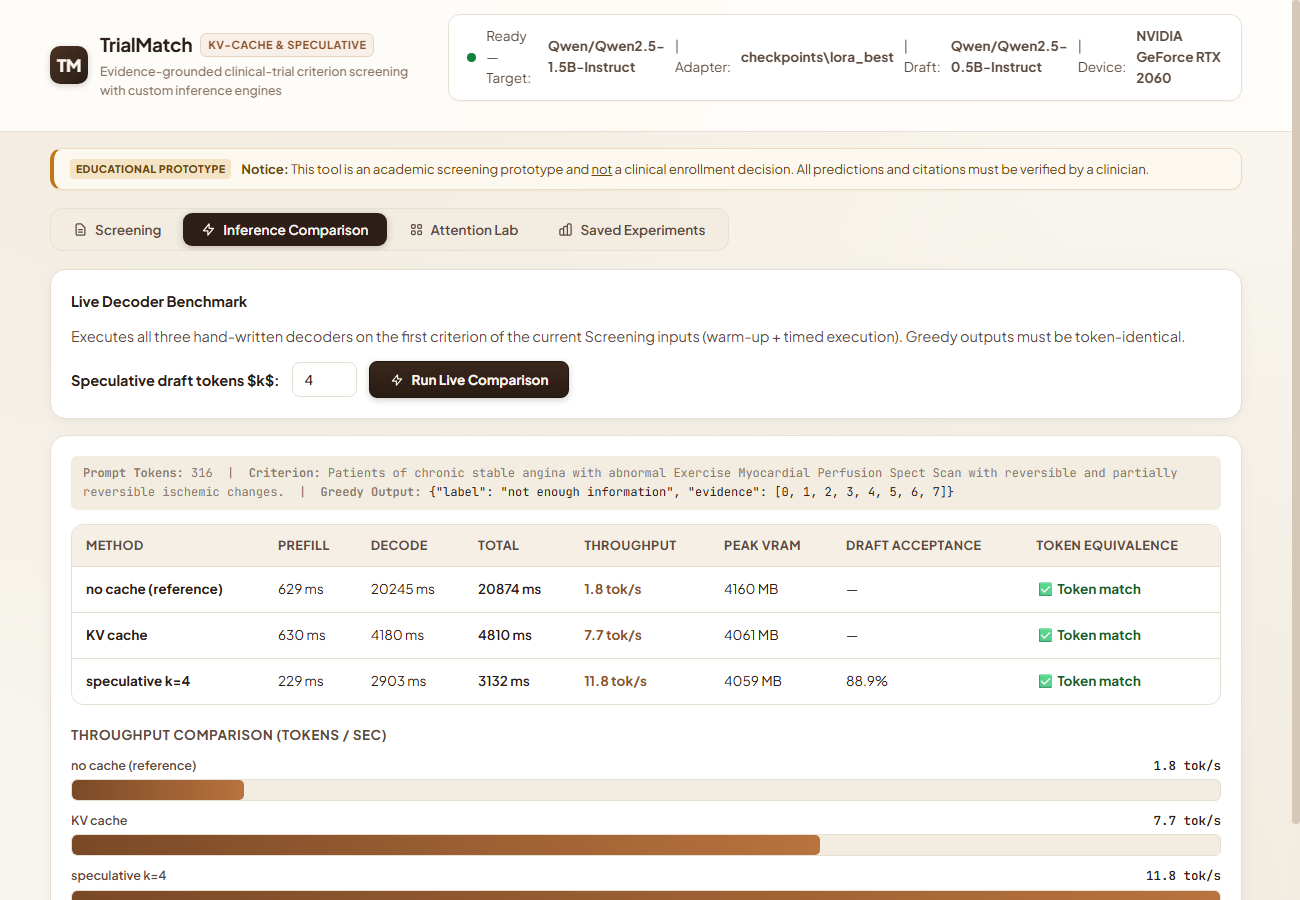
\includegraphics[width=\columnwidth]{app_bench.png}
\caption{Inference-comparison tab: live run of the three decoders on a real prompt (316 prompt tokens). Outputs are token-identical.}\label{fig:appbench}
\end{figure}

\section{Experimental Setup and Metrics}
Hardware: NVIDIA GeForce RTX 2060 (6\,GB, laptop-class, WDDM driver), 12-thread CPU, Windows 11, PyTorch 2.11 (CUDA 12.8), Transformers 5.6, PEFT 0.21. All inference is fp16 with greedy decoding and at most 64 new tokens for classification; benchmarks use fixed output lengths with the end-of-sequence token ignored in \emph{all} methods so they emit the same number of tokens. Timing uses one warm-up run, then the median of three CUDA-synchronised runs; peak memory is \texttt{torch.cuda.max\_memory\_allocated}. Because the 0.5B draft remains resident, \emph{peak memory in all rows includes both models}. Classification uses accuracy, macro-F1, per-class precision/recall/F1 and confusion matrices overall and separately per criterion type; macro-F1 averages over all classes of the label set (a class with no support and no correct prediction contributes 0). Evidence metrics are described in Sec.~III-D.

\section{Results and Discussion}\label{sec:results}
\subsection{Fine-tuning and before/after comparison}
Table~\ref{tab:train} and Fig.~\ref{fig:train} show v2 training. Training loss falls from 0.16 to 0.025 over four epochs. Validation \emph{loss} is lowest after epoch~1 and noisy afterwards, but validation generation quality behaves differently: macro-F1 climbs from 0.49 (epoch~1) to 0.59 (epoch~3) and falls slightly at epoch~4, so loss alone is a poor selector for this imbalanced task and we select epoch~3 by validation macro-F1. Training took about 37 minutes for four epochs on the RTX 2060 (peak 4.34\,GB).

\begin{figure}[t]
\centering
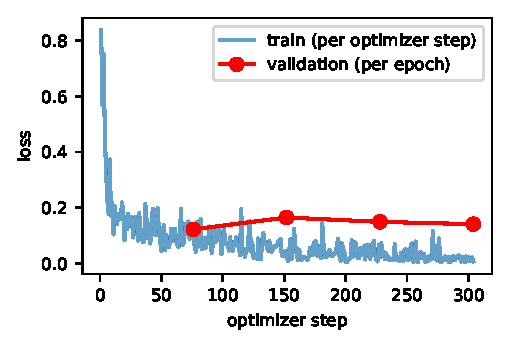
\includegraphics[width=\columnwidth]{training_curve.pdf}
\caption{v2 training and validation loss.}\label{fig:train}
\end{figure}

\begin{table}[t]
\centering
\caption{v2 training log (balanced sampling, 4 epochs). Validation accuracy, macro-F1 and evidence micro-F1 come from generation on the validation split; epoch 3 has the best validation macro-F1 and is the final adapter.}
\label{tab:train}
\footnotesize
\begin{tabular}{rrrrrrr}
\toprule
Epoch & Train loss & Val loss & Val Acc & Val mF1 & Val Ev-F1 & Min \\
\midrule
1 & 0.1613 & 0.1224 & 0.762 & 0.492 & 0.461 & 7 \\
2 & 0.0707 & 0.1648 & 0.699 & 0.560 & 0.473 & 16 \\
3 & 0.0417 & 0.1492 & 0.772 & 0.592 & 0.561 & 26 \\
4 & 0.0253 & 0.1409 & 0.743 & 0.582 & 0.538 & 37 \\
\bottomrule
\end{tabular}
\end{table}


Table~\ref{tab:cls} compares, on identical examples with identical prompts and greedy decoding, the base model, the first adapter (v1) and the final adapter (v2). The base model has essentially no task competence (accuracy 0.141 on validation, 0.223 on test; exclusion accuracy $\approx0$). Both adapters reach about 0.72 test accuracy, but accuracy hides a large difference: 91 of the 131 test exclusion criteria are \emph{not excluded}, so always answering that label already gives 0.695 exclusion accuracy, which is what v1 does. v2 trades some of this ``free'' accuracy for coverage of rare classes: test macro-F1 rises from 0.379 (v1) to 0.486 (v2), and validation macro-F1 from 0.349 to 0.592. Test accuracy is unchanged (0.723 vs.\ 0.718). \emph{Disclosure:} v1 was evaluated on the test split before v2 was designed, so the \emph{decision} to try class balancing was motivated by v1's test behaviour; however the balancing scheme, number of epochs and epoch choice for v2 were all fixed using validation data only, and v2 was run on the test split once.

\begin{table*}[t]
\centering
\caption{Criterion classification before/after fine-tuning (identical examples, greedy decoding, fp16, max 64 new tokens). Macro-F1 is over all label classes of the group (classes with zero support count as 0).}
\label{tab:cls}
\footnotesize
\begin{tabular}{llrrrrrr}
\toprule
Split & Model & Acc & mF1 & Inc Acc & Inc mF1 & Exc Acc & Exc mF1 \\
\midrule
val & Base (zero-shot) & 0.141 & 0.130 & 0.409 & 0.216 & 0.014 & 0.007 \\
val & v1: LoRA, loss-selected & 0.723 & 0.349 & 0.727 & 0.372 & 0.721 & 0.210 \\
val & v2: LoRA, balanced, F1-selected & 0.772 & 0.592 & 0.682 & 0.377 & 0.814 & 0.677 \\
test & Base (zero-shot) & 0.223 & 0.211 & 0.613 & 0.393 & 0.000 & 0.000 \\
test & v1: LoRA, loss-selected & 0.723 & 0.379 & 0.773 & 0.415 & 0.695 & 0.205 \\
test & v2: LoRA, balanced, F1-selected & 0.718 & 0.486 & 0.720 & 0.587 & 0.718 & 0.346 \\
\bottomrule
\end{tabular}
\end{table*}


Table~\ref{tab:perclass} and the confusion matrices (Fig.~\ref{fig:cm}) give the v2 detail. For inclusion criteria \emph{included} (F1 0.80) and \emph{not enough information} (0.78) remain strong, and \emph{not applicable} (3 cases) and \emph{not included} (7 cases) are now sometimes predicted (F1 0.50 and 0.27). For exclusion criteria, \emph{not excluded} (F1 0.83) still dominates, but the model now also outputs \emph{not enough information} (F1 0.18; 3 of 28 correct) and \emph{not applicable} (F1 0.38; 3 of 12 correct). \emph{Excluded} has zero test support, so its precision and recall are counted as 0 in macro-F1, which therefore understates exclusion macro-F1 (0.346; the metric files also report macro-F1 over present classes only). Still, 25 of 28 exclusion criteria with insufficient information are wrongly called \emph{not excluded}, so the model remains over-confident. With only 603 training examples (8 \emph{excluded} exclusion examples) rebalancing can only do so much, and confidence intervals are wide at this test size.

\begin{figure}[t]
\centering
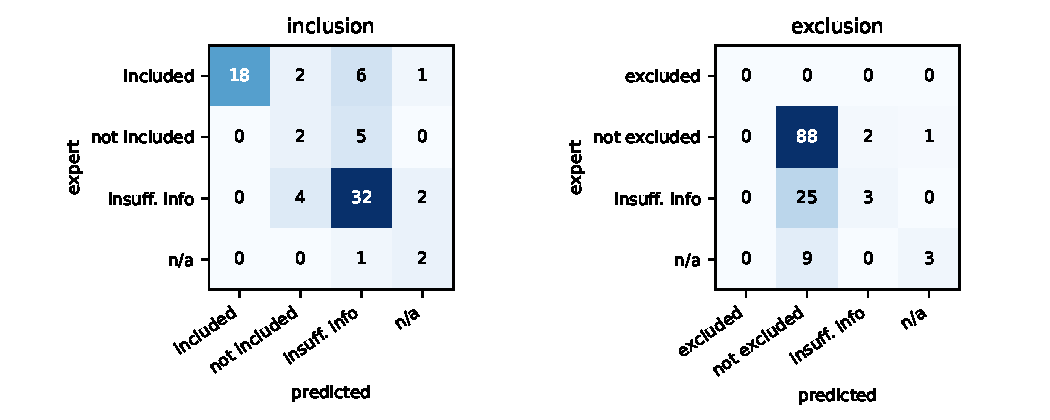
\includegraphics[width=\columnwidth]{confusion.pdf}
\caption{Test confusion matrices of the final (v2) model for inclusion (left) and exclusion (right) criteria.}\label{fig:cm}
\end{figure}

\begin{table}[t]
\centering
\caption{Per-class precision/recall/F1 of the fine-tuned model on the held-out test split.}
\label{tab:perclass}
\footnotesize
\begin{tabular}{llrrrr}
\toprule
Group & Class & P & R & F1 & Support \\
\midrule
inclusion & included & 0.800 & 0.889 & 0.842 & 27 \\
inclusion & not included & 0.000 & 0.000 & 0.000 & 7 \\
inclusion & not enough information & 0.756 & 0.895 & 0.819 & 38 \\
inclusion & not applicable & 0.000 & 0.000 & 0.000 & 3 \\
exclusion & excluded & 0.000 & 0.000 & 0.000 & 0 \\
exclusion & not excluded & 0.695 & 1.000 & 0.820 & 91 \\
exclusion & not enough information & 0.000 & 0.000 & 0.000 & 28 \\
exclusion & not applicable & 0.000 & 0.000 & 0.000 & 12 \\
\bottomrule
\end{tabular}
\end{table}


\subsection{Evidence retrieval}
Table~\ref{tab:evidence} reports sentence-ID retrieval. The base model cites many sentences (recall 0.89 but precision 0.08 on test). v1 is selective (test micro-F1 0.495) but nearly silent on exclusion criteria (recall 0.094): the expert evidence for \emph{not excluded} is usually empty, and v1 learned to emit empty lists there. v2 cites more and is better balanced: test micro-F1 0.543 (P 0.431, R 0.734), with exclusion recall rising from 0.094 to 0.594 and inclusion recall 0.806. The macro-all and macro-NE columns separate the effect of records with empty gold sets, which are 60\% of the data and count as perfect when the model also abstains.

\begin{table}[t]
\centering
\caption{Evidence-sentence retrieval. Micro: pooled counts. Macro-all: per-record mean with both-empty counted as 1.0; Macro-NE: only records with at least one gold sentence. $n_{NE}$ = number of such records.}
\label{tab:evidence}
\footnotesize
\begin{tabular}{lllrrrrrr}
\toprule
Split & Model & Group & P$_\mu$ & R$_\mu$ & F1$_\mu$ & F1$_{M}$ & F1$_{NE}$ & $n_{NE}$ \\
\midrule
val & Base & overall & 0.080 & 0.896 & 0.146 & 0.138 & 0.315 & 90 \\
val & Base & inclusion & 0.157 & 0.940 & 0.269 & 0.255 & 0.336 & 50 \\
val & Base & exclusion & 0.045 & 0.833 & 0.085 & 0.082 & 0.289 & 40 \\
val & Fine-tuned & overall & 0.453 & 0.591 & 0.513 & 0.738 & 0.578 & 90 \\
val & Fine-tuned & inclusion & 0.422 & 0.687 & 0.523 & 0.647 & 0.654 & 50 \\
val & Fine-tuned & exclusion & 0.537 & 0.458 & 0.494 & 0.781 & 0.483 & 40 \\
test & Base & overall & 0.079 & 0.894 & 0.144 & 0.109 & 0.369 & 61 \\
test & Base & inclusion & 0.146 & 0.952 & 0.254 & 0.222 & 0.370 & 45 \\
test & Base & exclusion & 0.038 & 0.781 & 0.072 & 0.045 & 0.367 & 16 \\
test & Fine-tuned & overall & 0.471 & 0.521 & 0.495 & 0.793 & 0.546 & 61 \\
test & Fine-tuned & inclusion & 0.500 & 0.742 & 0.597 & 0.664 & 0.684 & 45 \\
test & Fine-tuned & exclusion & 0.250 & 0.094 & 0.136 & 0.866 & 0.156 & 16 \\
\bottomrule
\end{tabular}
\end{table}


\subsection{Error analysis}
Of 206 test predictions of the final model, 58 are wrong (Table~\ref{tab:errors}). The largest group (25) is \emph{unsupported eligibility}: gold says \emph{not enough information}, the model asserts \emph{not excluded}. Examples: annotations 391 (``Intravenous corticosteroids within 3 months prior to the first dose''), 315 (``BMI $>$ 40 kg/m$^2$'') and 412 (``Vaccination within 4 weeks''): the note never mentions these facts, yet the model treats absence of evidence as proof of eligibility, the dangerous failure mode. Thirteen are over-abstentions although information exists, e.g.\ annotation 187 (respiratory-rate criterion, gold \emph{included} from sentence 2; the model cites the right sentence but abstains) and 185 (``diagnosed with shock, ARDS, or both'', gold \emph{included}). Ten are missed \emph{not applicable} cases such as annotation 751 (``breast-feeding'') and 683 (``previous tonsillectomy''), where the criterion is irrelevant to the patient but the model answers \emph{not excluded}. Ten are polarity errors, e.g.\ annotation 383 (active SLE symptoms; gold \emph{included}, predicted \emph{not included} despite citing the gold sentences 0 and 1), 691 (``symptoms of OSA, including snoring and sleepiness'', gold \emph{included}) and 835 (``Negative allergy skin test'': gold \emph{not enough information}, predicted \emph{not included} citing sentence~1), which show that correct sentence selection does not guarantee correct reasoning. These 12 representative cases (3 per type; full list in \texttt{results/error\_analysis.md}) cover contradictory cases and failures from missing information. Compared with v1 (57 errors) the number of errors is similar; balancing mostly converted unsupported-eligibility errors into over-abstentions and polarity errors.

\begin{table}[t]
\centering
\caption{Error taxonomy on the test split (final v2 model, 58 errors).}\label{tab:errors}
\footnotesize
\begin{tabular}{lr}
\toprule
Error type & Count\\
\midrule
Unsupported eligibility (missing info treated as met) & 25\\
Over-abstention although information exists & 13\\
Missed not-applicable & 10\\
Contradiction / wrong polarity & 10\\
\bottomrule
\end{tabular}
\end{table}

\subsection{KV-cache correctness and performance}
Table~\ref{tab:kv} (Fig.~\ref{fig:dec}, left) compares the uncached reference with our KV decoder on three prompt lengths (316, 488, 768 tokens) and three output lengths (16, 64, 128). Greedy tokens are identical in all nine configurations, so no mismatch investigation was necessary; this includes the real classification prompts, where outputs are short. Cached decoding is 2.0--8.1$\times$ faster in total time, with the gain growing with input and output length as the uncached cost grows quadratically while the cached decode step is constant-time per token. Prefill is similar for both (both process the prompt once). Peak memory is lower with the cache (4016--4167\,MB vs.\ 4101--4432\,MB) because the reference materialises full-sequence logits ($T\times$vocabulary) at every step. One cell (768 input, 128 output) shows 38.7$\times$: the uncached run took $\approx$547\,s versus 14\,s. This reproduced across two complete benchmark runs, so it is not a one-off, but we did not isolate the cause; plausible explanations are GPU memory pressure from the large uncached logits tensors or driver-level effects on the WDDM 6\,GB laptop GPU, and we therefore treat that single speed-up as an unexplained outlier and do not extrapolate from it. Absolute decode speed ($\approx$16 tokens/s) is low because each step is dominated by kernel-launch overhead in eager PyTorch for a small batch.

\begin{figure}[t]
\centering
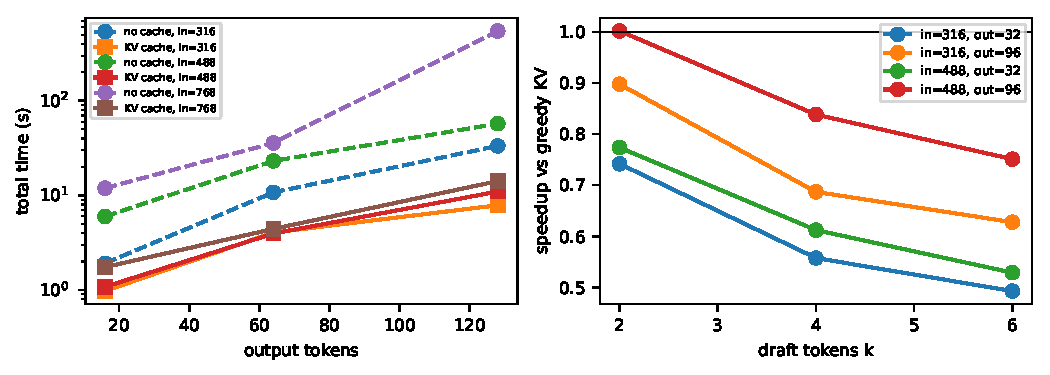
\includegraphics[width=\columnwidth]{decoding_bench.pdf}
\caption{Left: total generation time, cached vs.\ uncached (log scale). Right: speculative-decoding speed-up vs.\ greedy KV decoding for $k\in\{2,4,6\}$ (below 1 is a slowdown).}\label{fig:dec}
\end{figure}

\begin{table}[t]
\centering
\caption{Uncached reference vs. custom KV-cache greedy decoding (median of 3 timed runs after warm-up, CUDA-synchronised). Pre/Dec = prefill/decode seconds; peak memory includes the resident target and draft weights ($\approx$3.9\,GB).}
\label{tab:kv}
\footnotesize
\begin{tabular}{rrlrrrrrrrr}
\toprule
In & Out & Equal & Pre$_0$ & Dec$_0$ & Pre$_{kv}$ & Dec$_{kv}$ & tok/s$_0$ & tok/s$_{kv}$ & MB$_0$ & MB$_{kv}$ \\
\midrule
316 & 16 & yes & 0.12 & 1.79 & 0.11 & 0.86 & 8.4 & 16.5 & 4101 & 4016 \\
316 & 64 & yes & 0.12 & 10.63 & 0.11 & 3.93 & 6.0 & 15.8 & 4130 & 4016 \\
316 & 128 & yes & 0.12 & 33.21 & 0.11 & 7.74 & 3.8 & 16.3 & 4166 & 4016 \\
488 & 16 & yes & 0.23 & 5.76 & 0.18 & 0.90 & 2.7 & 14.9 & 4202 & 4074 \\
488 & 64 & yes & 0.24 & 22.87 & 0.18 & 3.77 & 2.8 & 16.2 & 4230 & 4074 \\
488 & 128 & yes & 0.25 & 57.02 & 0.51 & 10.37 & 2.2 & 11.7 & 4266 & 4074 \\
768 & 16 & yes & 0.83 & 11.09 & 0.83 & 0.91 & 1.3 & 9.2 & 4364 & 4167 \\
768 & 64 & yes & 0.39 & 35.27 & 0.57 & 3.74 & 1.8 & 14.5 & 4393 & 4167 \\
768 & 128 & yes & 3.52 & 543.81 & 3.56 & 10.59 & 0.2 & 9.0 & 4432 & 4167 \\
\bottomrule
\end{tabular}
\end{table}


\subsection{Tiled attention validation}
Table~\ref{tab:attn-err} shows that the tiled implementation agrees with the reference within the stated tolerances in all cases (shapes include $T_q<T_k$, a single query against a 100-token cache, and causal and non-causal masks, with block sizes 16 and 64 chosen so that tiles do not divide the sequence length). Table~\ref{tab:attn-perf} and Fig.~\ref{fig:attn} report cost on the GPU. The tiled kernel needs only 6.8\,MB of extra memory at $T{=}2048$ versus 580\,MB for the reference (an $85\times$ reduction, since score tiles stay $128\times128$), but it is \emph{much slower} (126.7\,ms vs.\ 15.7\,ms) and PyTorch's fused SDPA is fastest (0.58\,ms). This is expected: our version is a Python loop of many small matmul/elementwise kernels, each paying launch overhead and writing intermediates to global memory, whereas a fused kernel keeps tiles in on-chip SRAM and fuses the rescaling; at these sizes the reference's single large matmul is efficient and its memory is not yet limiting. The educational implementation therefore demonstrates correctness and the memory property, not speed.

\begin{figure}[t]
\centering
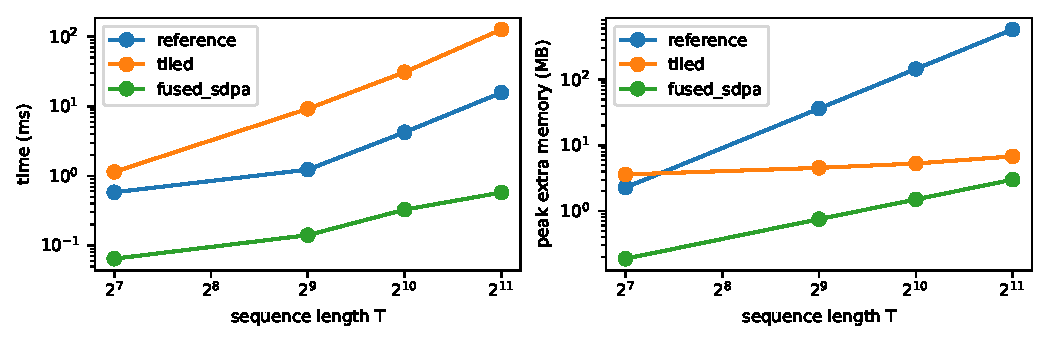
\includegraphics[width=\columnwidth]{attention_bench.pdf}
\caption{Attention runtime (left) and peak extra memory (right) versus sequence length.}\label{fig:attn}
\end{figure}

\begin{table}[t]
\centering
\caption{Numerical agreement with the reference attention over 6 shapes $\times$ causal/non-causal $\times$ 2 block sizes (incl. $T_q<T_k$ KV-cache shapes). Tolerance: $10^{-4}$ (fp32), $2\cdot10^{-2}$ (fp16).}
\label{tab:attn-err}
\footnotesize
\begin{tabular}{llrrrr}
\toprule
Variant & dtype & Cases & Max err & Mean err & Pass \\
\midrule
tiled & float32 & 24 & 8.34e-07 & 2.72e-08 & 24/24 \\
fused SDPA & float32 & 12 & 7.15e-07 & 3.49e-08 & 12/12 \\
tiled & float16 & 24 & 4.88e-04 & 4.51e-08 & 24/24 \\
fused SDPA & float16 & 12 & 1.95e-03 & 2.75e-05 & 12/12 \\
\bottomrule
\end{tabular}
\end{table}

\begin{table}[t]
\centering
\caption{Attention runtime and peak extra memory (12 heads, d=64, causal, fp16, cuda).}
\label{tab:attn-perf}
\scriptsize
\setlength{\tabcolsep}{3pt}
\begin{tabular}{lrrrrrr}
\toprule
T & Ref ms & Tiled ms & SDPA ms & Ref MB & Tiled MB & SDPA MB \\
\midrule
128 & 0.58 & 1.14 & 0.06 & 2.3 & 3.6 & 0.2 \\
512 & 1.23 & 9.20 & 0.14 & 36.3 & 4.5 & 0.8 \\
1024 & 4.23 & 30.84 & 0.33 & 145.0 & 5.3 & 1.5 \\
2048 & 15.67 & 126.74 & 0.58 & 580.1 & 6.8 & 3.0 \\
\bottomrule
\end{tabular}
\end{table}


\subsection{Speculative decoding}
Table~\ref{tab:spec} reports acceptance statistics, latency, throughput and memory for $k\in\{2,4,6\}$ on two prompts and two output lengths. Token equality with greedy target decoding holds in \emph{all} 12 settings, and our output also equals that of Hugging Face assisted generation (Table~\ref{tab:hf}); an initial mismatch against the library was traced to our reference call using \texttt{min\_new\_tokens} (which suppresses the end-of-sequence token that our loops do not suppress), not to the algorithm. Acceptance is 0.41--0.83 and falls as $k$ grows, as expected since later draft tokens depend on earlier ones. Nevertheless every setting is slower than plain greedy KV decoding, between 0.49$\times$ and 1.00$\times$ (Fig.~\ref{fig:dec}, right). The reason is cost, not correctness: with 24 vs.\ 28 layers the draft is not much cheaper per step than the target on this launch-bound GPU (target decode $\approx$60\,ms/token), so $k$ sequential draft steps cost nearly $k$ target steps, while verification adds a multi-token target pass and cache crop/catch-up overhead; speculative decoding only wins when draft steps are far cheaper than target steps and acceptance is high. Our draft is also the untuned 0.5B base-instruct model, so acceptance on the fine-tuned model's JSON outputs is imperfect; a fine-tuned or much smaller draft would likely help but was not evaluated. Peak memory is essentially unchanged (draft is resident in all runs).

\begin{table*}[t]
\centering
\caption{Custom greedy speculative decoding vs. greedy KV decoding of the target (Qwen2.5-1.5B + LoRA; draft Qwen2.5-0.5B). Acc = draft acceptance rate; Tok/Fwd = tokens committed per target forward; speedup $<1$ is a slowdown.}
\label{tab:spec}
\footnotesize
\begin{tabular}{rrlrrrrrrrrr}
\toprule
In & Out & k & Equal & Acc & Tok/Fwd & Greedy s & Spec s & Speedup & tok/s$_{greedy}$ & tok/s$_{spec}$ & MB \\
\midrule
316 & 32 & k=2 & yes & 0.64 & 2.29 & 1.84 & 2.48 & 0.74 & 17.4 & 12.9 & 4013 \\
316 & 32 & k=4 & yes & 0.45 & 2.67 & 1.84 & 3.31 & 0.56 & 17.4 & 9.7 & 4013 \\
316 & 32 & k=6 & yes & 0.41 & 3.20 & 1.84 & 3.74 & 0.49 & 17.4 & 8.6 & 4013 \\
316 & 96 & k=2 & yes & 0.71 & 2.40 & 5.87 & 6.54 & 0.90 & 16.4 & 14.7 & 4013 \\
316 & 96 & k=4 & yes & 0.54 & 3.10 & 5.87 & 8.55 & 0.69 & 16.4 & 11.2 & 4013 \\
316 & 96 & k=6 & yes & 0.49 & 3.84 & 5.87 & 9.35 & 0.63 & 16.4 & 10.3 & 4013 \\
488 & 32 & k=2 & yes & 0.64 & 2.29 & 2.03 & 2.62 & 0.77 & 15.8 & 12.2 & 4070 \\
488 & 32 & k=4 & yes & 0.43 & 2.67 & 2.03 & 3.32 & 0.61 & 15.8 & 9.7 & 4070 \\
488 & 32 & k=6 & yes & 0.41 & 3.20 & 2.03 & 3.84 & 0.53 & 15.8 & 8.3 & 4070 \\
488 & 96 & k=2 & yes & 0.83 & 2.67 & 5.96 & 5.95 & 1.00 & 16.1 & 16.1 & 4070 \\
488 & 96 & k=4 & yes & 0.67 & 3.69 & 5.96 & 7.11 & 0.84 & 16.1 & 13.5 & 4070 \\
488 & 96 & k=6 & yes & 0.61 & 4.57 & 5.96 & 7.94 & 0.75 & 16.1 & 12.1 & 4070 \\
\bottomrule
\end{tabular}
\end{table*}

\begin{table}[t]
\centering
\caption{Reference check against Hugging Face assisted generation (4 assistant tokens): token equality with our greedy output and wall time next to our $k{=}4$ implementation.}
\label{tab:hf}
\footnotesize
\begin{tabular}{rrrrr}
\toprule
In & Out & HF = ours & HF s & Ours k=4 s \\
\midrule
316 & 32 & yes & 3.72 & 3.31 \\
316 & 96 & yes & 10.56 & 8.55 \\
488 & 32 & yes & 3.72 & 3.32 \\
488 & 96 & yes & 8.15 & 7.11 \\
\bottomrule
\end{tabular}
\end{table}


\section{Limitations}
\begin{itemize}
\item The test split has only 8 patients and 206 criteria; many classes have 0--12 examples, so per-class metrics are very noisy and macro-F1 differences of a few points are not significant. We report a single training run (seed 42) without confidence intervals.
\item Even the final v2 model is over-confident on exclusion criteria (25 of 28 insufficient-information cases called \emph{not excluded}) and never predicts \emph{excluded} (0 test support); accuracy mostly reflects label skew. Only one rebalancing scheme (square-root class sampling) was tried, and v1 was evaluated on the test split before v2 was designed (Sec.~V-A).
\item Model candidates other than Qwen2.5-1.5B were not trained, so the model choice is feasibility-based, not empirically compared; hyper-parameters were not searched beyond the sampling scheme and the epoch count (selected by validation macro-F1 for v2, by validation loss for v1).
\item The 547\,s uncached outlier is unexplained; timings come from a single laptop GPU with eager PyTorch, so ratios may differ on other hardware, and speculative decoding was never faster here.
\item Explanations in the application are templated from the label and cited sentences rather than free-text reasoning; the system is an educational screening prototype and must not be used for enrollment decisions.
\item Greedy equality between cached/speculative and uncached decoding was observed in fp16 on tested inputs; it is not guaranteed in general because of floating-point non-associativity.
\end{itemize}

\section{Conclusion}
A 1.5B open-weight Transformer fine-tuned with LoRA on 603 patient-grouped criterion annotations improves accuracy from 0.22 to 0.72 on held-out patients and learns to localise evidence. Plain fine-tuning collapses to the majority class on exclusion criteria (macro-F1 0.38); class-balanced sampling with validation-macro-F1 selection raises macro-F1 to 0.49 and evidence F1 to 0.54, but the model remains over-confident when information is missing. The inference components were implemented from first principles and validated: cached decoding is token-identical and up to 8$\times$ faster, tiled online-softmax attention is numerically correct and 85$\times$ lighter in memory at $T=2048$ though slower than fused kernels, and speculative decoding is exactly equivalent to greedy decoding but slower on this hardware. The browser application makes the full workflow, evidence and decoder comparison available without code.

\section*{Appendix: AI-Use Statement}
Claude Code (Anthropic, Claude Sonnet 5.5) assisted with writing and debugging code, the application and this manuscript. All code was executed, tests and benchmarks were run on the author's machine and all numbers in the tables are generated from the logged result files by \texttt{scripts/make\_tables.py}. Libraries used: PyTorch, Hugging Face Transformers and PEFT, scikit-learn, FastAPI. The author is responsible for the submission and must be able to explain every component.

\begin{thebibliography}{10}
\bibitem{jin2024trialgpt} Q.~Jin \emph{et al.}, ``Matching patients to clinical trials with large language models,'' \emph{Nature Communications}, vol.~15, art.~9074, 2024.
\bibitem{hu2022lora} E.~J. Hu \emph{et al.}, ``LoRA: Low-rank adaptation of large language models,'' in \emph{Proc. ICLR}, 2022.
\bibitem{qwen25} A.~Yang \emph{et al.}, ``Qwen2.5 technical report,'' arXiv:2412.15115, 2024.
\bibitem{vaswani2017attention} A.~Vaswani \emph{et al.}, ``Attention is all you need,'' in \emph{Proc. NeurIPS}, 2017.
\bibitem{su2021roformer} J.~Su \emph{et al.}, ``RoFormer: Enhanced Transformer with rotary position embedding,'' arXiv:2104.09864, 2021.
\bibitem{milakov2018online} M.~Milakov and N.~Gimelshein, ``Online normalizer calculation for softmax,'' arXiv:1805.02867, 2018.
\bibitem{dao2022flashattention} T.~Dao \emph{et al.}, ``FlashAttention: Fast and memory-efficient exact attention with IO-awareness,'' in \emph{Proc. NeurIPS}, 2022.
\bibitem{kwon2023pagedattention} W.~Kwon \emph{et al.}, ``Efficient memory management for large language model serving with PagedAttention,'' in \emph{Proc. SOSP}, 2023.
\bibitem{leviathan2023speculative} Y.~Leviathan, M.~Kalman, and Y.~Matias, ``Fast inference from Transformers via speculative decoding,'' in \emph{Proc. ICML}, 2023.
\bibitem{chen2023accelerating} C.~Chen \emph{et al.}, ``Accelerating large language model decoding with speculative sampling,'' arXiv:2302.01318, 2023.
\end{thebibliography}

\end{document}
